% Created 2025-09-18 Thu 17:43
% Intended LaTeX compiler: lualatex
\documentclass[a4paper,12pt]{article}
\usepackage{amsmath}
\usepackage{fontspec}
\usepackage{graphicx}
\usepackage{longtable}
\usepackage{wrapfig}
\usepackage{rotating}
\usepackage[normalem]{ulem}
\usepackage{capt-of}
\usepackage{hyperref}
\usepackage{luacode}
\usepackage[french]{babel}
\usepackage{microtype}
\usepackage[autolanguage]{numprint}
\npthousandsep{~}
\usepackage{bxtexlogo}
\bxtexlogoimport{*}
\bxtexlogoimport{**}
\usepackage{fontspec}
\usepackage{ulem}
\usepackage{soul}
\setmainfont{Source Serif 4}[Path=/home/anthea/org/fonts/Source_Serif_4/static/, UprightFont=SourceSerif4-Regular.ttf, ItalicFont=SourceSerif4-Italic.ttf, BoldFont=SourceSerif4-Bold.ttf, BoldItalicFont=SourceSerif4-BoldItalic.ttf]
\setsansfont{Source Sans 3}[Path=/home/anthea/org/fonts/Source_Sans_3/static/, UprightFont=SourceSans3-Regular.ttf, ItalicFont=SourceSans3-Italic.ttf, BoldFont=SourceSans3-Bold.ttf, BoldItalicFont=SourceSans3-BoldItalic.ttf]
\setmonofont{JetBrains Mono}[Path=/home/anthea/org/fonts/JetBrains_Mono/static/, UprightFont=JetBrainsMono-Regular.ttf, ItalicFont=JetBrainsMono-Italic.ttf, BoldFont=JetBrainsMono-Bold.ttf, BoldItalicFont=JetBrainsMono-BoldItalic.ttf]
\renewcommand{\familydefault}{\sfdefault}
\usepackage[usenames,dvipsnames,svgnames,table]{xcolor}
\definecolor{customgray}{HTML}{505050}
\usepackage[top=3.2cm, bottom=3.2cm, left=2.4cm, right=2.4cm]{geometry}
\usepackage[cm]{fullpage}
\usepackage{setspace,fancyhdr,indentfirst,lastpage,datetime,authblk,ifthen,etoolbox,titling}
\singlespacing
\pagestyle{fancy}
\fancyhf{}
\fancyfoot[C]{\thepage\ / \pageref{LastPage}}
\renewcommand{\headrulewidth}{0pt}
\setlength{\parindent}{0pt}
\setcounter{secnumdepth}{3}
\setlength{\columnsep}{0.8cm}
\setlength{\marginparwidth}{1.6cm}
\setcounter{page}{1}
\usepackage{csquotes}
\usepackage{array,booktabs,multirow,tabularx,colortbl,diagbox,makecell,ltablex,adjustbox,multicol}
\usepackage{enumitem}\setlist{nosep}\setlist[itemize]{leftmargin=*}
\usepackage[toc,page]{appendix}
\usepackage[nottoc]{tocbibind}
\newenvironment{keyword}{\begin{trivlist}\item[]{\bfseries Mots-clés :}}{\end{trivlist}}
\usepackage{graphicx,caption,wrapfig}
\usepackage[most,breakable,xparse,listings,skins]{tcolorbox}
\usepackage[colorinlistoftodos]{todonotes}
\usepackage{newfloat}
\DeclareFloatingEnvironment[fileext=lol,listname={\vspace{-2em}},name=Listing]{listing}
\captionsetup{format=plain,font=small,labelfont=bf}
\captionsetup[listing]{labelfont=bf,textfont=it}
\usepackage{fvextra,amsfonts,amssymb,amsmath,mathrsfs,mathtools,stmaryrd}
\usepackage{algorithm2e}
\usepackage{pgf,tikz,pgfplots,pgfplotstable,arydshln,subcaption,forest}
\pgfplotsset{compat=1.18}
\usepackage[acronym]{glossaries}
\makenoidxglossaries
\usepackage{url,orcidlink,hyperref}
\hypersetup{colorlinks=true, linkcolor=customgray, citecolor=customgray, urlcolor=customgray, pdfborder={0 0 0}, unicode=true}
\bxtexlogoimport{*}
\bxtexlogoimport{**}
\author{Cyprien PIERRE \orcidlink{0009-0009-9040-6795}}
\date{2025-09-18}
\title{quickDoc\\\medskip
\large An ergonomic lightweight markup language with mnemonic inspirations for writing all kind of documents}
\hypersetup{
 pdfauthor={Cyprien PIERRE \orcidlink{0009-0009-9040-6795}},
 pdftitle={quickDoc},
 pdfkeywords={},
 pdfsubject={},
 pdfcreator={},
 pdflang={French}}
\usepackage[style=backend=biber,style=iso-numeric,citestyle=numeric-comp,doi=true,isbn=true,mincrossrefs=2,autocite=superscript]{biblatex}
\addbibresource{~/org/references.bib}
\begin{document}

\maketitle
\begin{abstract}
Abstract
\end{abstract}

\textbf{Mots clés : }\keywords{Mots clés}
\section{Introduction}
\label{sec:orgef1d8bc}

\begin{verbatim}
parler en revue de litérature de l'avantage des LML // LaTeX et // word
\end{verbatim}

\begin{verbatim}
parler des problématiques d'incohérences et des specs non rigides
\end{verbatim}

\begin{verbatim}
parler des limites actuelles
\end{verbatim}
\section{Etat de l'art}
\label{sec:org329d5a4}
Il existe de multiples approches à la production de documents formatés. L'utilisation de logiciels de traitement de texte tels que MS Word, Google Docs ou encore Only Office est probablement la voies la plus largement répendue. Ces solutions proposent des environnements graphiques qui présentent aux utilisateurs les modifications qu'ils peuvent apporter à leurs document. Cette approche a des limitation notamment dans la réalisations de documents exécutable \footnote{\textbf{Document exécutable :} Désigne un document dont des éléments sont executé (p. ex. code) et remplacés par le produit de l'exécution (p. ex. schéma ou diagrammes).}.

Une autre approche très répendue est d'écrire le formatage du texte en même temps que le contenu. Cette seconde approche implique généralement l'utilisation d'un éditeur de texte comme Neovim, Emacs, iA Writter, etc. associé à un logiciel adapté à la convention de rédaction choisie par l'utilisateur. De manière générale, l'utilisateur utilisera un langage de balisage pour déclarer le formatage.

Il existe ainsi deux grandes catégories de langages de balisages appliqués à la rédaction de documents : les langages formels (\TeX{}, HTML, TEI\ldots{}) et les langages informels (Markdown, Org-Mode, AsciiDoc\ldots{})\autocite{leonardGuidanceMarkdownDesign2016}. Cette seconde catégorie constitue la famille des  (\protect\hyperlink{gls-1}{\label{gls-1-use-1}LML}).
\subsection{Langages de définition de documents}
\label{sec:orgcb60bc5}
Le standard actuel de rédaction de documents aux mises en formes rigoureuse est \TeX{}. Il s'agit à la fois un langage de programmation et un logiciel d'impression de document. Pour l'utiliser lors de la rédaction de document nous utilisons un format de rédaction tels que \LaTeX{}, ConTeXt, Texinfo, ou encore OpTeX. Ces formats emploient des macros \TeX{} pour faciliter la mise en page. Le format le plus répendu, nottament dans le monde académique, est le \LaTeX{}. La production d'un fichier \TeX{} prêt à être exporté (en PDF, DVI, HTML, PostScript\ldots{}) requiert une ou plusieurs étapes de compilation du texte source. Les compilateurs (ou moteurs) les plus fréquents sont pdfTeX, LuaTeX, et XeTeX et ils utilisent respectivement les variantes \LaTeX{} que sont pdfLaTeX, LuaLaTeX et XeLaTeX. Ces variantes sont similaires à \LaTeX{} avec des fonctions complémentaires adaptées au moteur choisis. \LaTeX{} bénéficie d'extensions communautaires compatibles ou spécialisées à un moteur et permettant de créer programmatiquement les documents. Nous pouvons citer ici les paquets XyMTeX pour dessiner des structures moléculaires, Biber pour générer les bibliographies, TikZ pour réaliser tout type de dessins ou encore ArabTeX qui permet la prise en charge des langues arabes. Pour rédiger des documents \LaTeX{}, il est nécessaire d'installer une distribution \TeX{}. La plus connue est \TeX{} Live dont il existe de multiples dérivés et pour les utilisateurs de Windows il semblerait que MikTeX soit apprécié. Enfin, l'emploi d'un éditeur (Emacs avec AUCTeX, le logiciel LyX, ou encore l'application web Overleaf) facilite la rédaction grace à des fonctionnalités d'assistance et de précomplétion. Des projets comme LTeX+\autocite{LtexplusLtexlsplus2025}  et Writefull\autocite{Writefull} permettent de porter ces techniques d'assistances dans d'autres logiciels.

A la lecture de ce descriptif nous remarquons que la production de document avec \LaTeX{} implique en de multiples endroits de réaliser des choix et des arbitrages avant même de commencer à rédiger. Quel compileur utiliser ? Quels sont les extensions les plus à jours ou les plus stables ? Dans quel environnement vais-je travailler ? etc. Ces considérations persistent durant tout le processus de rédaction ce qui entraine des périodes de déconcentration et parasite le travail de l'utilisateur. Ce constat semble inciter à la création d'un système probablement plus restreint mais résiliant. 

\begin{verbatim}
Parler de Typst/Quatro et de Scribble (lisp)
\end{verbatim}
\subsection{Langages de balisage léger}
\label{sec:orgf12d34a}
Markdown est le \protect\hyperlink{gls-1}{\label{gls-1-use-2}LML} le plus populaire mais aussi le plus critiqué. Sa définition simple (MD Basics) en fait un langage très facile d'approche, facile à apprendre par tout individu. Ses faiblaisses résident néanmoins de la diversité de ses implémentations. MD Basic est supporté de façon homogène mais n'inclus pas l'ensemble des usages textuels possibles. Ces ommissions ont tendu à la création de douzaines de dérivés non cohérents entres eux. Les utilisateurs sont donc contraint d'apprendre plusieurs Markdown selon l'environnement dans lequel ils rédigent leurs documents.

\begin{verbatim}
Parler de RestructuredText, de Org-Mode et AsciiDoc au minimum
\end{verbatim}

Org-mode, dont le document Orgdown décris la synthaxe, est un \protect\hyperlink{gls-1}{\label{gls-1-use-3}LML} très respecté par les utilisateurs d'Emacs. Ce langage est bien plus structuré que le Markdown et offre de nombreuses possibilités grâce à son étroite intégration avec \LaTeX{} et les macros d'Emacs. Son intrication profonde avec Emacs le rend difficilement portable à d'autres environnements de rédaction.

AsciiDoc est une référence majeure des \protect\hyperlink{gls-1}{\label{gls-1-use-4}LML}. Il bénéficie d'une gouvernance de projet communautaire éprouvée, administrée par l'Eclipse Foundation. Ce langage couvre probablement tous les besoins de rédaction existant. Sa documentation est riche mais peut être intimidante pour un nouvel utilisateur.
\subsection{Emergence d'un besoin}
\label{sec:org3b4e94e}
=> Specify (github)
=> LLM
=> CBE

conclusion : création de \textbf{quickDoc}
\section{Syntaxe}
\label{sec:orgdb802e5}
\subsection{Définition}
\label{sec:orgd58cfb7}
Un bloc de texte est constituée d'une ligne continue et de la première ligne vide immédiatement en dessous. Un retour chario n'entraine alors pas de création d'un nouveau bloc.
\subsection{Balisage}
\label{sec:orgdfd852b}
Le texte d'un bloc peut être formaté au niveau d'une lettre, d'un mot, d'une ligne continue ou d'un ensemble de ligne continue espacées entres elles d'un unique retour chariot.

Le formattage se réalise en entourant \emph{explicitement} le contenu à formater par les balises de formatage. Ces balises sont des symboles textuels accessibles facilement sur un clavier. Le tableau \ref{tab:org5687a90} liste les balises utilisées par \textbf{quickDoc} et présente 3 des modalitées d'emplois. Il existe une tollérance pour le formatage d'une ligne complète, comme l'ensemble de la ligne est formatée jusqu'au retour chariot alors il convient d'apposer \emph{uniquement} une double marque en début de ligne.  

\begin{longtable}{llllll}
\caption{\label{tab:org5687a90}Liste des balisages}
\\
\hline
Type & Balise & HTML5 & Une lettre & Un mot & Une ligne\\
\hline
\endfirsthead
\multicolumn{6}{l}{Suite de la page précédente} \\
\hline

Type & Balise & HTML5 & Une lettre & Un mot & Une ligne \\

\hline
\endhead
\hline\multicolumn{6}{r}{Suite page suivante} \\
\endfoot
\endlastfoot
\hline
Superscript & \texttt{+} &  & \texttt{+l+etter} & \texttt{+word+} & \texttt{++ this is a superscripted line}\\
Subscript & \texttt{-} &  & \texttt{-l-etter} & \texttt{-word-} & \texttt{-{}-{} this is a subscripted line}\\
Strique & \texttt{\textasciitilde{}} &  & \texttt{\textasciitilde{}l\textasciitilde{}etter} & \texttt{\textasciitilde{}word\textasciitilde{}} & \texttt{\textasciitilde{}\textasciitilde{}\textasciitilde{}this is a striked line}\\
Highlight & \texttt{=} &  & \texttt{=l=etter} & \texttt{=word=} & \texttt{== this is an highlighted line}\\
Comment & \texttt{;} &  & \texttt{;l;etter} & \texttt{;word;} & \texttt{;; this is a commented line}\\
Bold & \texttt{*} & <strong> & \texttt{*l*etter} & \texttt{*word*} & \texttt{** this is a bolded line}\\
Italique & \texttt{/} & <em> & \texttt{/l/etter} & \texttt{/word/} & \texttt{// this is an italicised line}\\
Underline & \texttt{\_} &  & \texttt{\_l\_etter} & \texttt{\_word\_} & \texttt{\_\_ this is an underlined line}\\
Verbatim & \texttt{:} &  & \texttt{:l:etter} & \texttt{:word:} & \texttt{:: this is a line of verbatim}\\
Math & \texttt{\$} &  & \texttt{\$l\$etter} & \texttt{\$word\$} & \texttt{\$\$ this is a line of math}\\
Code & \texttt{`} &  & \texttt{`l`etter} & \texttt{`word`} & \texttt{`` this is a line of code}\\
\hline
\end{longtable}

La mise en forme d'un ensemble de ligne continues est réalisée par l'inscription de trois balises à la ligne précédent et celle suivant le texte à mettre en forme. Cette mise en forme est valide pour toutes les marques pour des raisons d'uniformité synthaxique bien que certains formatages n'ai que peu de raisons d'être employés de la sorte. La création d'un formatage multiligne se construit de la manière suivante :
\begin{multicols}{2}
\begin{verbatim}
```<parametres>
 <code
 sur plusieurs
 lignes>
```
\end{verbatim}

\begin{verbatim}
;;; <parametres>
 <commentaires
 sur plusieurs
 lignes>
;;;
\end{verbatim}

\begin{verbatim}
$$$ <parametres>
 <formule mathématique
 sur plusieurs
 lignes>
$$$
\end{verbatim}

\begin{verbatim}
::: <parametres>
 <formule mathématique
 sur plusieurs
 lignes>
:::
\end{verbatim}
\end{multicols}

Les blocs de codes peuvent être configurer de manière à obtenir plusieurs comportements. Les paramètres sont à inscrire sous la forme \texttt{[[[set <parameter-name>:<value>]]]} avec les parametres suivants :
\begin{itemize}
\item \texttt{lang} : défini le langage utilisé pour le formatage du texte,
\item \texttt{runtime} : défini le moteur d'éxecution le cas échéant et si pertinent (e.g. deno, node, bun, etc.).
\item \texttt{play} : autorise l'execution du code avec \texttt{t} et l'empêche par défaut (\texttt{nil}).
\item \texttt{export} : précise ce qui doit être imprimé lors de l'export. Ce paramètre peut prendre spécifiquement les valeurs suivantes :
\begin{itemize}
\item \texttt{verbatim} : imprime le code en police monospace avec son formatage et coloration synthaxique,
\item \texttt{result} : remplace le bloc de code avec son résultat (e.g. un graphique, un tableau, etc.),
\item \texttt{both} : imprime successivement le code en verbatim puis son résultat,
\item \texttt{neither} : n'imprime rien.
\end{itemize}
\end{itemize}

Un exemple complet de bloc de code : \breakline
\texttt{`` [[[set lang:python export:result]]] import matplotlib.pyplot as plt; plt.plot([1, 2, 3], [4, 5, 6]); plt.show()}

\begin{center}
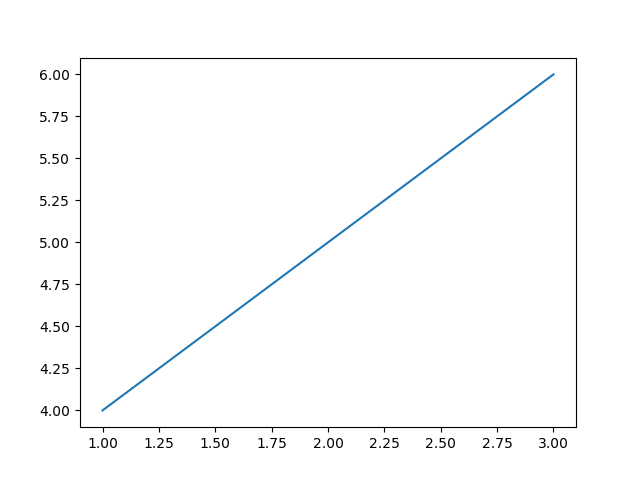
\includegraphics[width=.9\linewidth]{./quickDoc-exemple-code.png}
\end{center}

\newline
Les blocs de commentaires sont de 4 types :
\begin{itemize}
\item sans précision, ils ne sont pas exportées
\item avec \texttt{type:todo-inline} ils impriment un bloc de type "TODO" en lieu et place ten que celui ci : \todo[inline]{bloc "TODO" en ligne}
\item avec \texttt{type:todo} ils impriment un bloc de type "TODO" dans la marge du document tel que celui ci : \todo{e.g.}
\item avec \texttt{type:properties} il permet de créer une liste de propriétées pour le bloc associée tel que :
\begin{verbatim}
Ceci est un bloc de texte avec des propriétées attachées.
;; [[[set type:properties key1:value1 key2:value2]]]
\end{verbatim}
\end{itemize}
\newline
Les blocs de mathématiques peuvent être associées à un résolveur d'équation tel que :
\texttt{\$\$ [[[set solver:<nom du résolveur>]]] <equation>}
Quelques exemples de résolveurs : Math.js, SymPy, Maxima, SageMath, Wolfram Alpha, etc.
\newline
Les blocs verbatims peuvent être mis en forme en renseignant un type en lieu et place du <parametres> sous la forme \texttt{[[[set type:<value>]]]}. Ces types de blocs s'appellent des \emph{admonitions}\autocite{donathAdmonitionsMaterialMkDocs} et peuvent prendre les valeurs suivantes : note, abstract, info, tip, success, question, warning, failure, danger, bug, exemple, quote, keywords, answer, hypothesis, theorem, proof.

Les verbatims peuvent également être utilisés pour collecter des entrées utilisateurs et créer des formulaires en écrivant \texttt{:[[[get <property> <key>:<value>]]]:} où \texttt{<key>} correspond au type attendu et \texttt{<value>} correspond à la contrainte associée. Par exemple, voici des appels d'entrées valides :
\begin{itemize}
\item \texttt{:[[[get user-name string:20]]]:} donnera \texttt{\_\_\_\_\_\_\_\_\_\_\_\_\_\_\_\_\_\_\_\_} et sera affecté à la propriété "user-name",
\item \texttt{:[[[get user-lang string:2]]]:} donnera \texttt{\_\_} et sera affecté à la propriété "user-lang".
\end{itemize}

Les balises peuvent être combinées entre elles dans les limites de la matrice de compatibilité présentée par le tableau \ref{tab:orgbbe6cb8}. La combinaison du superscript et du subscript produit un middlescript.

\begin{table}[htbp]
\caption{\label{tab:orgbbe6cb8}Compatibility matrix between formatings}
\centering
\begin{tabular}{lrlllllllllll}
\hline
Beacon Type & N° & 1 & 2 & 3 & 4 & 5 & 6 & 7 & 8 & 9 & 10 & 11\\
\hline
Highlight & 1 & x & \textcolor{green}{1} & \textcolor{green}{1} & \textcolor{green}{1} & \textcolor{green}{1} & \textcolor{green}{1} & \textcolor{green}{1} & \textcolor{green}{1} & \textcolor{green}{1} & \textcolor{red}{0} & \textcolor{red}{0}\\
Strike & 2 & \textcolor{green}{1} & x & \textcolor{green}{1} & \textcolor{green}{1} & \textcolor{green}{1} & \textcolor{green}{1} & \textcolor{green}{1} & \textcolor{green}{1} & \textcolor{green}{1} & \textcolor{red}{0} & \textcolor{red}{0}\\
Subscript & 3 & \textcolor{green}{1} & \textcolor{green}{1} & x & \textcolor{green}{1} & \textcolor{green}{1} & \textcolor{green}{1} & \textcolor{green}{1} & \textcolor{green}{1} & \textcolor{green}{1} & \textcolor{red}{0} & \textcolor{red}{0}\\
Superscript & 4 & \textcolor{green}{1} & \textcolor{green}{1} & \textcolor{green}{1} & x & \textcolor{green}{1} & \textcolor{green}{1} & \textcolor{green}{1} & \textcolor{green}{1} & \textcolor{green}{1} & \textcolor{red}{0} & \textcolor{red}{0}\\
Bold & 5 & \textcolor{green}{1} & \textcolor{green}{1} & \textcolor{green}{1} & \textcolor{green}{1} & x & \textcolor{green}{1} & \textcolor{green}{1} & \textcolor{green}{1} & \textcolor{red}{0} & \textcolor{red}{0} & \textcolor{red}{0}\\
Comment & 6 & \textcolor{green}{1} & \textcolor{green}{1} & \textcolor{green}{1} & \textcolor{green}{1} & \textcolor{green}{1} & x & \textcolor{green}{1} & \textcolor{green}{1} & \textcolor{red}{0} & \textcolor{red}{0} & \textcolor{red}{0}\\
Italique & 7 & \textcolor{green}{1} & \textcolor{green}{1} & \textcolor{green}{1} & \textcolor{green}{1} & \textcolor{green}{1} & \textcolor{green}{1} & x & \textcolor{green}{1} & \textcolor{red}{0} & \textcolor{red}{0} & \textcolor{red}{0}\\
Underline & 8 & \textcolor{green}{1} & \textcolor{green}{1} & \textcolor{green}{1} & \textcolor{green}{1} & \textcolor{green}{1} & \textcolor{green}{1} & \textcolor{green}{1} & x & \textcolor{red}{0} & \textcolor{red}{0} & \textcolor{red}{0}\\
Verbatim & 9 & \textcolor{green}{1} & \textcolor{green}{1} & \textcolor{green}{1} & \textcolor{green}{1} & \textcolor{red}{0} & \textcolor{red}{0} & \textcolor{red}{0} & \textcolor{red}{0} & x & \textcolor{red}{0} & \textcolor{red}{0}\\
Inline Math & 10 & \textcolor{red}{0} & \textcolor{red}{0} & \textcolor{red}{0} & \textcolor{red}{0} & \textcolor{red}{0} & \textcolor{red}{0} & \textcolor{red}{0} & \textcolor{red}{0} & \textcolor{red}{0} & x & \textcolor{red}{0}\\
Inline Code & 11 & \textcolor{red}{0} & \textcolor{red}{0} & \textcolor{red}{0} & \textcolor{red}{0} & \textcolor{red}{0} & \textcolor{red}{0} & \textcolor{red}{0} & \textcolor{red}{0} & \textcolor{red}{0} & \textcolor{red}{0} & x\\
\hline
\end{tabular}
\end{table}

Lists begins with a bullets that represent their meaning followed by a space. The following is supported :
\begin{itemize}
\item Ordered lists starts with \texttt{1.},
\item Unordered lists starts with \texttt{-},
\item Headers are lists too and starts with a \texttt{\#}, the number of \texttt{\#} set the level of the header.
\end{itemize}

Unordered lists and headers bullets can be followed by a multivalue key in the form of \texttt{[<state>:<priority>:<impact>]} with all optionnal values :
\begin{itemize}
\item a formal \texttt{<state>} : TODO, PLANED, DOING, PAUSE, DONE, ABORTED,
\item an estimated \texttt{<priority>} value : A, B, C, D, E,
\item an \texttt{<impact>} factor : 5, 4, 3, 2 ,1.
\end{itemize}

\begin{verbatim}
# [TODO:B:3] Title with a full key

  - [DOING:5] a task with a high impact factor
      - [ ] a check box action
      - [x] a checked check box action
\end{verbatim}

Sublevels (nested lists) are supported for headers, ordered and unordered lists. There must be 4 spaces before the sublevel bullet.

\begin{multicols}{3}
\begin{verbatim}
# First level header
    ## Second    
        ### Third
\end{verbatim}

\begin{verbatim}
- First unordered list
    - Second
        - Third
\end{verbatim}

\begin{verbatim}
1. First ordered list
    1.1. Second
        1.1.1. Third
\end{verbatim}
\end{multicols}

The export \protect\hyperlink{gls-2}{\label{gls-2-use-1}backend} shall provide settings to customise desired formatting outputs of ordered lists (alpha-numeric numbering, dots, parentheses\ldots{}) 
\subsection{Tags}
\label{sec:org15013c8}
Tous les blocs de textes peuvent être associées à des tags.
Un tag s'écrit \texttt{\#<tag>} peut être insérée à n'importe quel endroit du bloc de texte en respectant les rêgles de balisage décrites au paragraphe \ref{sec:orgdfd852b}.

\begin{center}
\begin{tabular}{lll}
\hline
Type & Lemma & Behavior\\
\hline
Ref Link & \texttt{@element} & Insère un \texttt{[[lien]]} unidirectionnel\\
Tag & \texttt{\#tag} & Insère un \texttt{[[lien]]} bidirectionnel\\
\hline
\end{tabular}
\end{center}

Les tags sont utilisés pour faire de l'analyse sémantique. Ecrire un tag entraine la création ou la mise à jour d'un fichier "tag\_<nom-du-tag>.qdo" constitué comme ceci :
\begin{verbatim}
# Nom-du-tag
[[[get count:?]]] ;; nombre d'occurence dans le projet
[[[get blocs:?nom-du-tag]]] ;; tous les blocs utilisants le tag
\end{verbatim}

L'instruction \texttt{[[[get blocs:?nom-du-tag]]]} peut être complété par un système de tris. Par exemple, pour lister les blocs par ordre de date décroissante on écrira \texttt{[[[get blocs:?nom-du-tag order-by:date-desc]]]}.

Un système de trâme permettant aux utilisateurs de préconfigurer ces documents et de modifier en lot leurs configuration serait un atoût en matière d'expérience utilisateur.
\subsection{Callouts}
\label{sec:org0ccae96}
Callouts are bidirectional links inside the current document. They are used to quickly jump to content, a reference, or a definition.

\begin{table}[htbp]
\caption{Text callouts}
\centering
\begin{tabular}{lll}
\hline
Type & Lemma & Behavior\\
\hline
Reference & \texttt{[ref:@entry]} & \\
Foot Note & \texttt{[fn:note]} & \\
Quote & \texttt{[cite:@entry]} & \\
Figure ref & \texttt{[fig:name]} & \\
Table ref & \texttt{[tbl:name]} & \\
Code ref & \texttt{[src:name]} & \\
Header jump & \texttt{[header]} & \\
\hline
\end{tabular}
\end{table}
\subsection{Links}
\label{sec:org2cf0a46}
Tous les liens suivent l'écriture \texttt{[[<CONTEXT>:<LINK>:<QUERY>][<TEXT>]]} pù seul le \texttt{<LINK>} \textbf{doit} être renseigné. Les autres éléments sont : 
\begin{itemize}
\item \texttt{<CONTEXT>} fournis des informations complémentaires pour l'affichage du lien. Cela permet de mettre en oeuvre des affichages adaptés aux images, vidéos, player de musique, flux RSS, etc.
\item \texttt{<LINK>} is the path of the resource on the World Wide Web, in a file system, or on any supported network. We can call a `Header ID` from the current document or from another one.
\item \texttt{<QUERY>} est utilisé pour renvoyer vers une section particulière du lien (un titre, un callout, etc.). Une requete s'écris \texttt{?[<key>:<value>]}, où la clé est n'importe quelle propriété et la valeur est n'importe quelle chaine de charactère.
\item \texttt{<TEXT>} est le texte de remplacement à afficher à la place du lien.
\end{itemize}


\begin{table}[htbp]
\caption{<LINK> types}
\centering
\begin{tabular}{lll}
\hline
Type & Lemma & Can be used to\\
\hline
URI &  & \\
Web URL & \texttt{[[https:link]]} & Display a bookmark\\
Local File & \texttt{[[file:<path>]]} & \\
Musique & \texttt{[[:<path or url>]]} & Display a music player\\
Image & \texttt{[[img:<path or url>]]} & \\
Document & \texttt{[[doc:<path or url>]]} & Display a document viewer\\
Video & \texttt{[[vid:<path or url>]]} & Display a video player\\
Header ID & \texttt{[[id:headerId]]} & \\
RSS Flow & \texttt{[[rss:<url>]]} & Display a list of last entries\\
IRC Flow & \texttt{[[irc:<url>]]} & Display a list of last messages\\
Email & \texttt{[[mailto:<email>]]} & Display a contact form\\
\hline
\end{tabular}
\end{table}
\subsection{Macroprogramme}
\label{sec:orga74100d}
Des utilisations avancées de documentation programmatique peuvent faire appel à des macros définies par l'utilisateur ou par la plateforme de service.

Dans quickDoc, ces macros sont appellées avec trois crochets tels que : \texttt{[[[<macro-name>]]]}

Elles sont définies par l'utilisateur comme ceci :
\begin{verbatim}
[[[defmacro <macro-name>
       <macro-code>
]]]
\end{verbatim}
\subsection{Configuration}
\label{sec:org562ce93}
One might consider using a separate file to manage, preserve, and share all its configurations.
That might be a file for \protect\hyperlink{gls-1}{\label{gls-1-use-5}LML} styles and tweaks, one for special export settings (e.g., \TeX{}, ODT, or HTML).
A good way to go is by declaring at the first line of the document 
\begin{verbatim}
;;[[[set config file:file1 file:file... file:fileN]]]
\end{verbatim}
\subsubsection{Text layout}
\label{sec:orgfdc0e8b}
First, define a style like
\begin{verbatim}
[[[set text_style name:paraghaphe scope:raw-text al:justif size:12 long:80char color:black font:source-sans-pro columns:nil]]]
\end{verbatim}

Then apply it, it will be set from the statement until the new one.
\begin{verbatim}
[[[use text-style name:paragraphe]]]
\end{verbatim}
\section{Consistency analysis}
\label{sec:org6fb774f}
A consistent lightweight markup language shall have only one way to format text.

Markdown variants on the \ref{tab:org79aea84} are limited to those listed by IANA's "Markdown Variant" \autocite{MarkdownVariants2023}. We exclude SSW and Quarto, the first one is too contextual and the second is based on Pandoc markdown.

\begin{table}[htbp]
\caption{\label{tab:org79aea84}Text formatting consistency versus Markdown variants}
\centering
\begin{tabular}{lrrrrrrrrrrrr}
\hline
Format & Bol & Ita & OrL & UnL & Und & Hig & Str & Ver & Cod & Sup & Sub & Com\\
\hline
quickDoc & 1 & 1 & 1 & 1 & 1 & 1 & 1 & 1 & 1 & 1 & 1 & 1\\
Common Markdown\autocite{johnmacfarlaneCommonMarkSpec2024} &  &  &  &  &  &  &  &  &  &  &  & \\
MultiMarkdown\autocite{fletchert.penneyMultiMarkdownUsersGuide2023} &  &  &  &  &  &  &  &  &  &  &  & \\
Github Flavored Markdown\autocite{GitHubFlavoredMarkdown2019} &  &  &  &  &  &  &  &  &  &  &  & \\
Pandoc\autocite{johnmacfarlanePandocUsersGuide2025} &  &  &  &  &  &  &  &  &  &  &  & \\
Fountain\autocite{SyntaxFountain} &  &  &  &  &  &  &  &  &  &  &  & \\
Markdown for RFCs\autocite{thomasleitnerKramdownSyntax} &  &  &  &  &  &  &  &  &  &  &  & \\
Pandoc2rfc &  &  &  &  &  &  &  &  &  &  &  & \\
Markdown Extra\autocite{PHPMarkdownExtra} &  &  &  &  &  &  &  &  &  &  &  & \\
Markedly Structured Text\autocite{JupyterbookMystmd2025} &  &  &  &  &  &  &  &  &  &  &  & \\
AsciiDoc &  &  &  &  &  &  &  &  &  &  &  & \\
reStructuredText &  &  &  &  &  &  &  &  &  &  &  & \\
Orgdown (Org-Mode) &  &  &  &  &  &  &  &  &  &  &  & \\
Textile &  &  &  &  &  &  &  &  &  &  &  & \\
Djot &  &  &  &  &  &  &  &  &  &  &  & \\
Wikitext &  &  &  &  &  &  &  &  &  &  &  & \\
Creole &  &  &  &  &  &  &  &  &  &  &  & \\
txt2tags &  &  &  &  &  &  &  &  &  &  &  & \\
Setext &  &  &  &  &  &  &  &  &  &  &  & \\
\hline
\end{tabular}
\end{table}
\begin{tablenotes}
\begin{multicols}{3}\small
\begin{itemize}
  \item Bol : Bold
  \item Ita : Italique
  \item OrL : Ordered List
  \item UnL : Unordered List
  \item Und : Underline
  \item Hig : Highlight
  \item Str : Strike
  \item Ver : Verbatim
  \item Cod : Inline code
  \item Sup : Superscript
  \item Sub : Subscript
  \item Com : Comment
\end{itemize}
\end{multicols}
\end{tablenotes}
\section{Capacity analysis}
\label{sec:org123507c}

\section{Typesystem compatibility}
\label{sec:org05f0891}
\section{Termes et définitions}
\label{sec:org2aaceb0}
\emph{Nous avons beau parler la même langue, nous ne parlons pas toujours le même langage.}
\begin{multicols}{3}
\subsection{Glossaire}
\label{sec:org270bb3e}
\textbf{\hypertarget{gls-5}{Backend}}\hspace*{1em}Couche logicielle gérant la logique métier, la gestion des données et la communication entre les applications\hspace*{.5em}\pageref{gls-2-use-1}
\subsection{Acronymes}
\label{sec:orgb16bc22}
\textbf{\hypertarget{gls-348}{LML}}\hspace*{1em}\hspace*{.5em}\pageref{gls-1-use-1}, \pageref{gls-1-use-2}, \pageref{gls-1-use-3}, \pageref{gls-1-use-4}, \pageref{gls-1-use-5}

\end{multicols}
\section{Références}
\label{sec:orga108136}
\printbibliography[heading=none]
\end{document}
